%%%%%%%%%%%%%%%%%%%%%%%%%%%%%%%%%%%%%%%%%
% FRI Data Science_report LaTeX Template
% Version 1.0 (28/1/2020)
% 
% Jure Demšar (jure.demsar@fri.uni-lj.si)
%
% Based on MicromouseSymp article template by:
% Mathias Legrand (legrand.mathias@gmail.com) 
% With extensive modifications by:
% Antonio Valente (antonio.luis.valente@gmail.com)
%
% License:
% CC BY-NC-SA 3.0 (http://creativecommons.org/licenses/by-nc-sa/3.0/)
%
%%%%%%%%%%%%%%%%%%%%%%%%%%%%%%%%%%%%%%%%%


%----------------------------------------------------------------------------------------
%	PACKAGES AND OTHER DOCUMENT CONFIGURATIONS
%----------------------------------------------------------------------------------------
\documentclass[fleqn,moreauthors,10pt]{ds_report}
\usepackage[english]{babel}

\graphicspath{{fig/}}




%----------------------------------------------------------------------------------------
%	ARTICLE INFORMATION
%----------------------------------------------------------------------------------------

% Header
\JournalInfo{FRI Natural language processing course 2023}

% Interim or final report
\Archive{Project report} 
%\Archive{Final report} 

% Article title
\PaperTitle{An Automatic Movie Summary Generator} 

% Authors (student competitors) and their info
\Authors{Luka Pavićević, Andrija Stanišić, Stefanela Stevanović}

% Advisors
\affiliation{\textit{Advisors: Slavko Žitnik}}

% Keywords
\Keywords{}
\newcommand{\keywordname}{Keywords}


%----------------------------------------------------------------------------------------
%	ABSTRACT
%----------------------------------------------------------------------------------------

\Abstract{
}

%----------------------------------------------------------------------------------------

\begin{document}

% Makes all text pages the same height
\flushbottom 

% Print the title and abstract box
\maketitle 

% Removes page numbering from the first page
\thispagestyle{empty} 

%----------------------------------------------------------------------------------------
%	ARTICLE CONTENTS
%----------------------------------------------------------------------------------------

\section*{Introduction}

In today's world, there is an abundance of films being produced every year. It can be difficult for audiences to keep up with all the latest releases. Movie fans often resort to reading summaries or synopses to get a sense of what a particular film is about before deciding whether or not to watch it. However, it can be a time-consuming and difficult task to manually summarise a long film script.

Here Natural Language Processing comes in. Through the use of Natural Language Processing techniques, we can automate the task of summarising film scripts, saving both time and effort.

In this project, our aim is to create a system that can accurately summarise film scripts into concise and informative synopses through the use of Natural Language Processing. By doing so, we hope to provide film enthusiasts with a quick and efficient way to get a sense of a film's plot, characters and key events. Ultimately, this will help them in their decision-making process when choosing which films to watch.


\section*{Related works}

One of the related works in text summarization is the work by Aleš Žagar and Marko  Robnik-Šikonja \cite{zagar2022}, who explored the use of various summarization approaches, including neural models, to produce short summaries from larger texts. In their work, they addressed the problem of selecting the most appropriate summarization model for a given text, and proposed a solution that uses a neural metamodel to automate the selection process based on the input document's representation. This work presents an innovative approach to text summarization, particularly in addressing the issue of model selection, which is important in ensuring the quality of generated summaries.

The article \cite{APARICIO20167} discusses the performance of generic text summarization algorithms on films and documentaries, using extracts from news articles produced by reference models of extractive summarization. The study aims to evaluate the quality of automatic summaries produced for films and documentaries, using well-known behaviors of news articles as a reference. Six text-based summarization approaches were used: Maximal Marginal Relevance (MMR), LexRank, Latent Semantic Analysis (LSA), Support sets, Key Phrase-based Centrality (KP-Centrality), and TextRank. The study found that LexRank and Support Sets had the best performance on movies of all the mentioned aproaches.

The paper \cite{DHARANIYA2023102150} proposes an ensemble deep learning model for generating movie scripts, which means that multiple models are combined to improve the accuracy and robustness of the system.  The model uses the Ensemble-based Movie Scrip Generation (EMCG), where the Optimized hybrid script generation process using ensemble learning is performed by Bi-LSTM, GPT3, and GPT Neo X models, where the parameters of deep learning algorithms are optimized using the AI-CMO algorithm.

\section*{Corpus}

For our project, we gathered data from various sources including scripts from IMSDb, summaries from Metacritic (MC) and Rotten Tomatoes (RT), as well as subtitles and summaries from Subslikescript (SLS). In addition to that, we also collected some other available data such as movie genres and year of release. Initially, we merged the IMSDb scripts with all other available data to create the first dataset. However, some of the scripts did not have corresponding summaries or subtitles. Therefore, we merged these scripts with whatever data was available for them. In the process of data cleaning, we identified that some of the subtitles contained an unreasonably low number of sentences, some having as few as one. As a result, we removed all subtitles containing less than 100 sentences. This left us with the following data set:
\begin{itemize}
  \item IMSDb Scripts: 943 entries
  \item Subslikescript Subtitles: 772 entries
  \item Subslikescript Summaries: 785 entries
  \item Metacritic Summaries: 835 entries
  \item Rotten Tomatoes Summaries: 781 entries
\end{itemize}

For this dataset we performed the corpus analysis, that is shown in table 1. 

\begin{table}[h]
\caption{Average, minimum and maximum number of sentences, words and TTR for the data in the first data set, collected from different sources.}
\begin{center}
\begin{tabular}{c|c|ccc}
  & DATA & AVG & MIN &  MAX\\
 \hline
  & IMSDb Scripts &  2807&  334  & 5345\\ 
  & SLS Subtitles &  1505& 121 & 11077 \\
Sentences & SLS Summaries&  4 & 1 & 22 \\
& MC Summaries &  2 & 1 & 12\\
& RT Summaries &  3 & 1 & 7 \\
 \hline
  & IMSDb Scripts &  29421& 4302  & 64311\\ 
  & SLS Subtitles &  11660& 718 & 49988 \\
Words & SLS Summaries&  123 & 12 & 616 \\
& MC Summaries &  64 & 10 & 320\\
& RT Summaries &  82 & 7 & 123 \\
\hline
  & IMSDb Scripts &  0.143&  0.071  & 0.312\\ 
  & SLS Subtitles &  0.157& 0.002 & 0.422 \\
TTR & SLS Summaries&  0.696 & 0.471 & 1.000 \\
& MC Summaries &  0.828 & 0.534 & 1.000\\
& RT Summaries &  0.757 & 0.600 & 1.000 \\
\end{tabular}
\label{tab1}
\end{center}
\end{table}

\begin{figure}[h]
\begin{center}
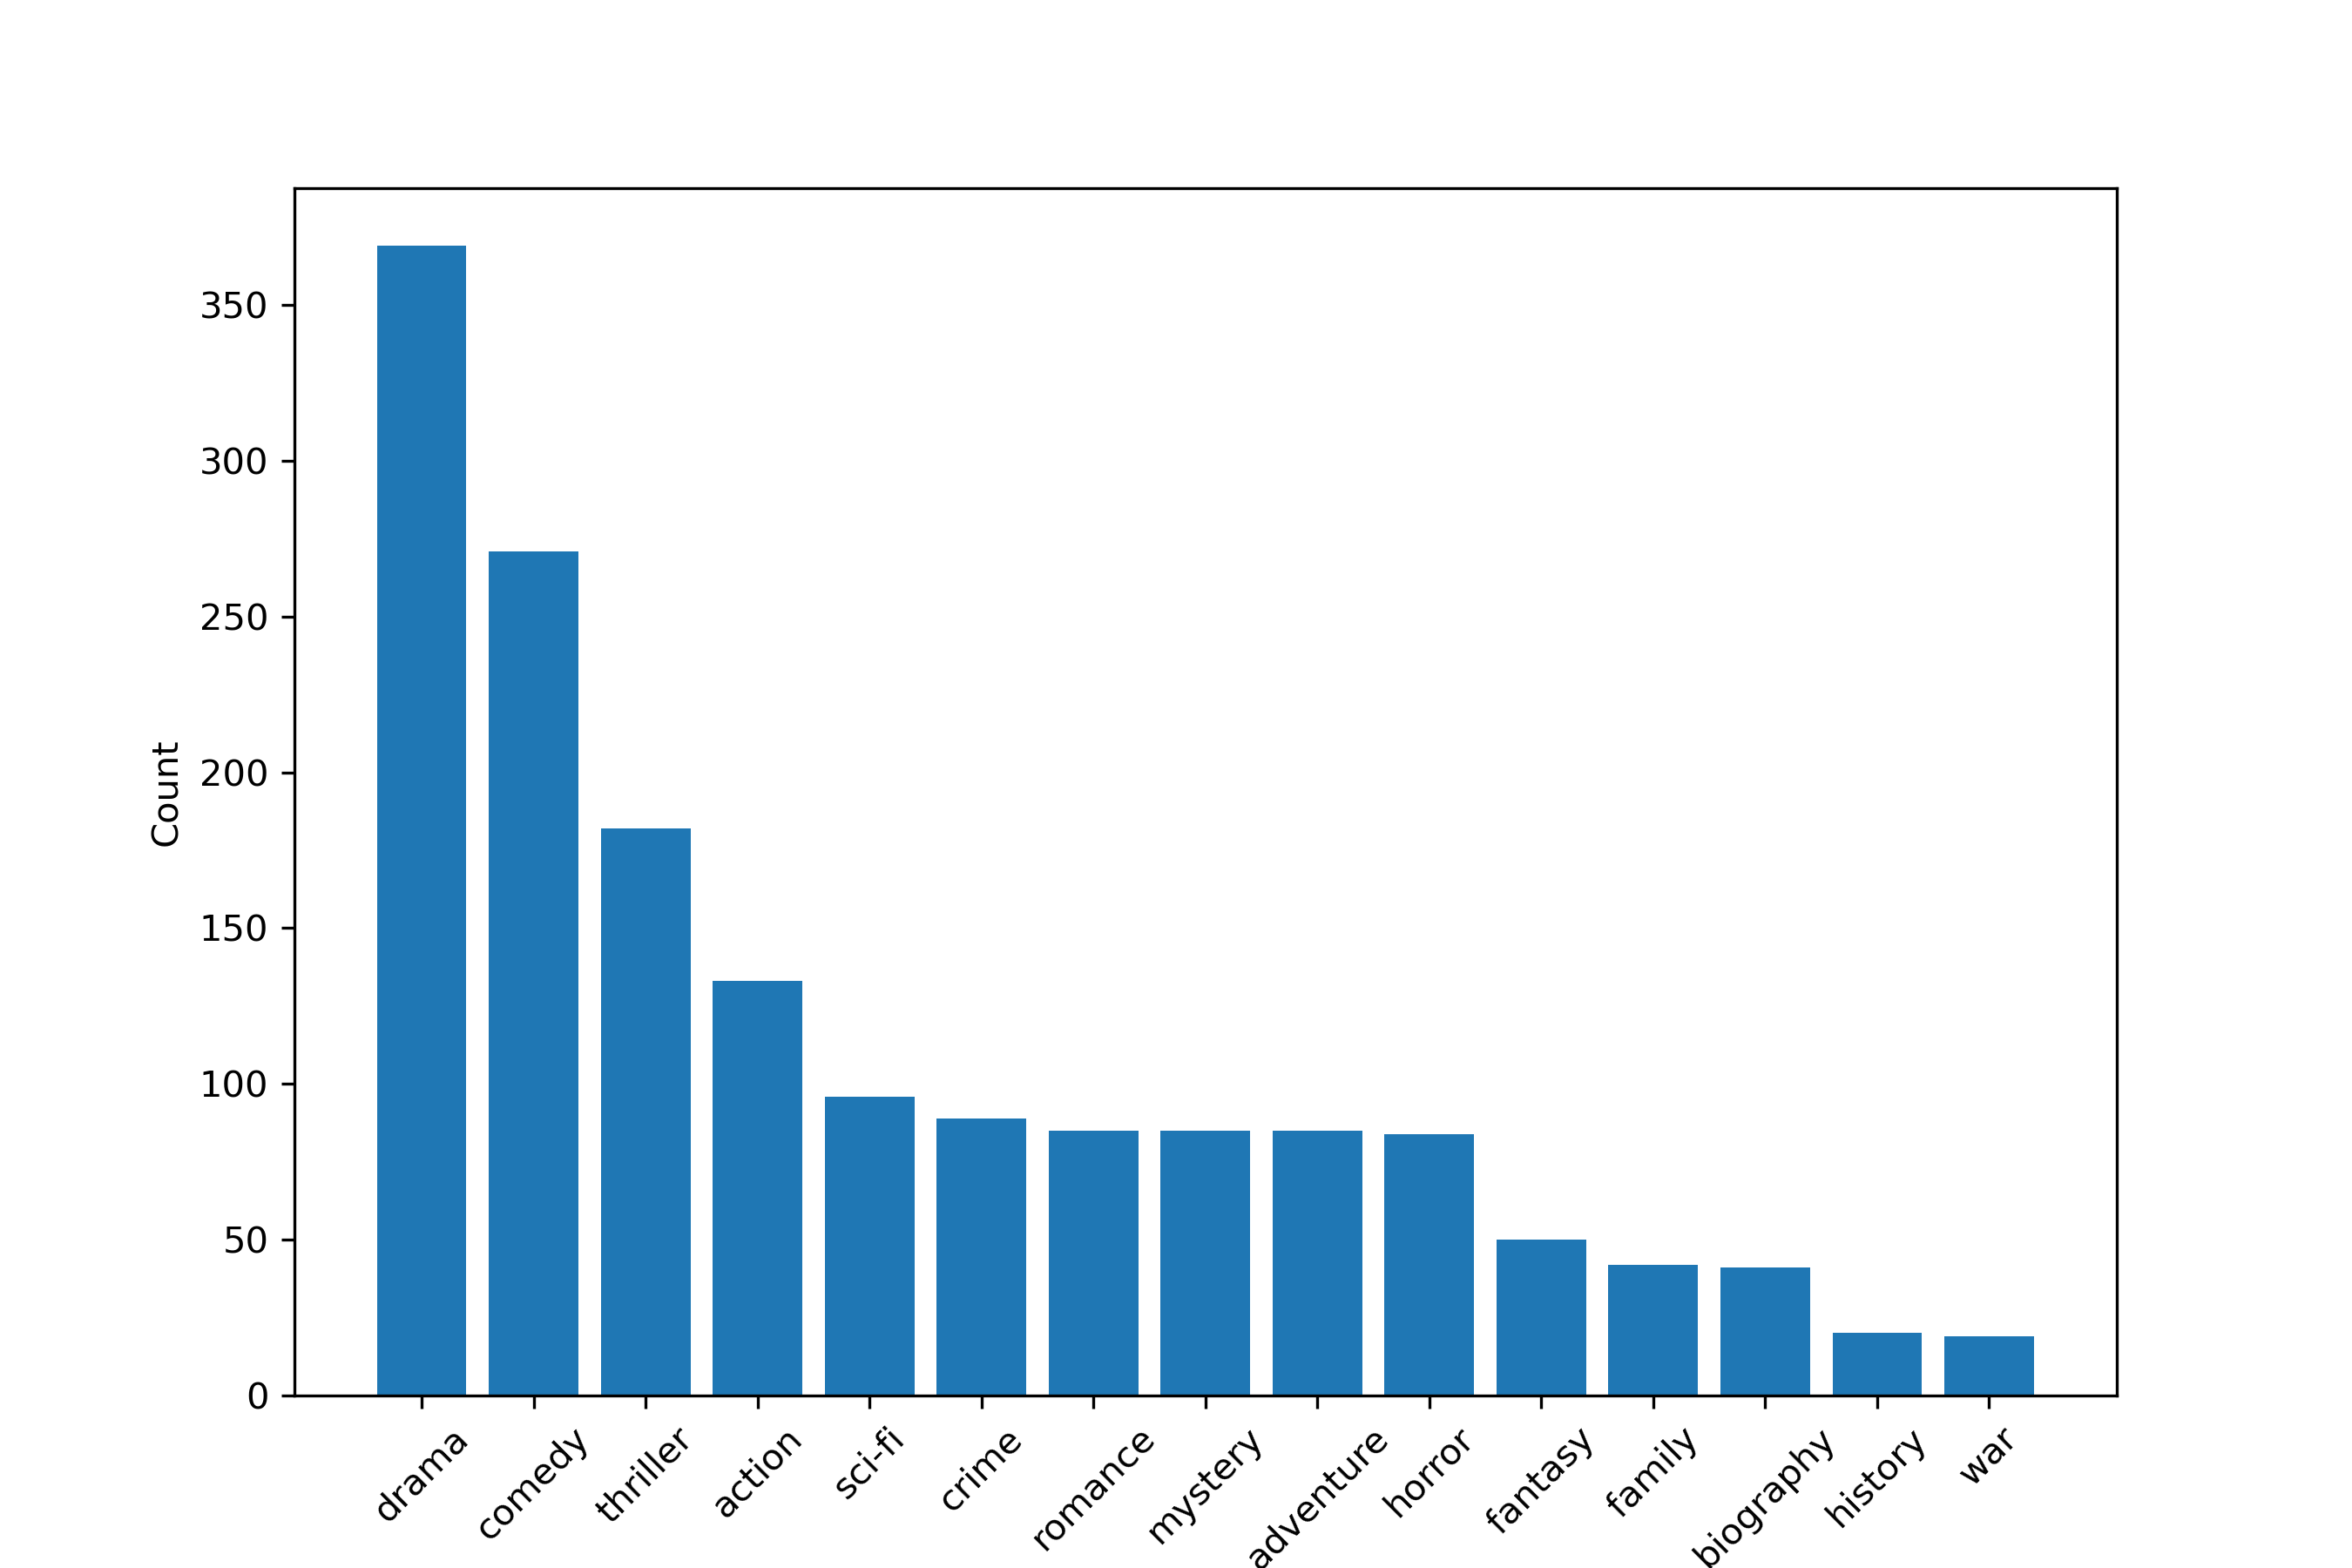
\includegraphics[width=1.0\columnwidth]{movie_genres.png}
\end{center}
\caption{Top 15 most common movie genres in our first data set. The most prevalent genre is drama, followed by comedy and thriller.}
\label{fig1}
\end{figure}

For our analysis, we utilized genre data available from Rotten Tomatoes and Metacritic. As each movie can belong to multiple genres, we performed an intersection between the genres from these two sites to obtain a more concise and accurate genre description for each movie. The objective was to avoid having too many genres associated with the same movie. Next, we counted the occurrence of each genre within the intersected movie genres, and plotted the 15 most common genres in Figure 1.



\section*{Baseline aproach}

As a baseline approach to summarizing the movie scripts in this project, we employ Latent Semantic Analysis (LSA). 

LSA is a popular text summarization technique that uses singular value decomposition (SVD) to reduce the dimensionality of a document-term matrix and capture the underlying semantic structure of the text. The model assumes that words with similar meanings will appear in similar contexts and can be grouped together.

To use the LSA model for text summarization, we split the movie scripts into scenes and preprocess the scene text by converting it to lowercase, removing non-alphanumeric characters from each sentence. We then use the Sumy library to tokenize the scene text and prepare it for input into the LSA model.

The LSA model identifies the most important sentences in a document based on their semantic similarity to other sentences. We use the LsaSummarizer module from Sumy to generate a summary of each scene, with a target of two sentences per scene.

After generating the summaries using LSA, we evaluate their quality using the ROUGE metric. ROUGE is a commonly used metric for evaluating text summarization models that measures the overlap between the generated summary and the reference summary. ROUGE provides multiple scores such as ROUGE-1, ROUGE-2, and ROUGE-L.

ROUGE-1 measures the overlap of unigrams (single words) between the generated and reference summaries. ROUGE-2 measures the overlap of bigrams (pairs of adjacent words) between the generated and reference summaries. ROUGE-L is a variant that computes the longest common subsequence between the generated and reference summaries, which can handle paraphrasing and word order differences.

The Fig. 2. shows the average ROUGE scores for each of the three metrics for each reference summary. We achieved decent scores for ROUGE-1 and ROUGE-L, bearing in mind that this is only a baseline model.  However, our model struggled to capture longer, more complex phrases and sentences, as reflected in the low score for ROUGE-2.

We believe that the poor performance on ROUGE-2 may be due to the fact that LSA is a bag-of-words model and does not capture word order or phrase structure. Additionally, the model may struggle with more complex sentences that contain multiple clauses or dependent phrases. Despite these limitations, our baseline approach with LSA provides a reasonable starting point for summarizing movie scripts and could be improved with further optimization and fine-tuning. 

\begin{figure}[h]
\begin{center}
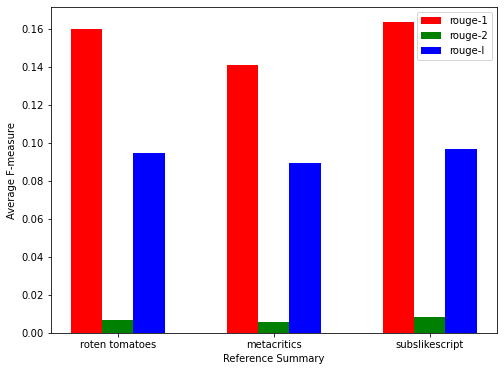
\includegraphics[width=1.0\columnwidth]{rouge_scores.png}
\end{center}
\caption{ROUGE Scores by Reference Summary}
\label{fig1}
\end{figure}




%----------------------------------------------------------------------------------------
%	REFERENCE LIST
%----------------------------------------------------------------------------------------
\bibliographystyle{unsrt}
\bibliography{report}


\end{document}